\chapter{Mattock: A modernized Open Computer Forensics Architecture}
This appendic tries to show the big picture of a prospect computer forensics framework that builds on both the good parts of the Open Computer Forensics Architecture (OCFA), and the concepts and sub-systems introduced in the research paper.  
\section{The OCFA architecture}
\begin{figure}
\centering
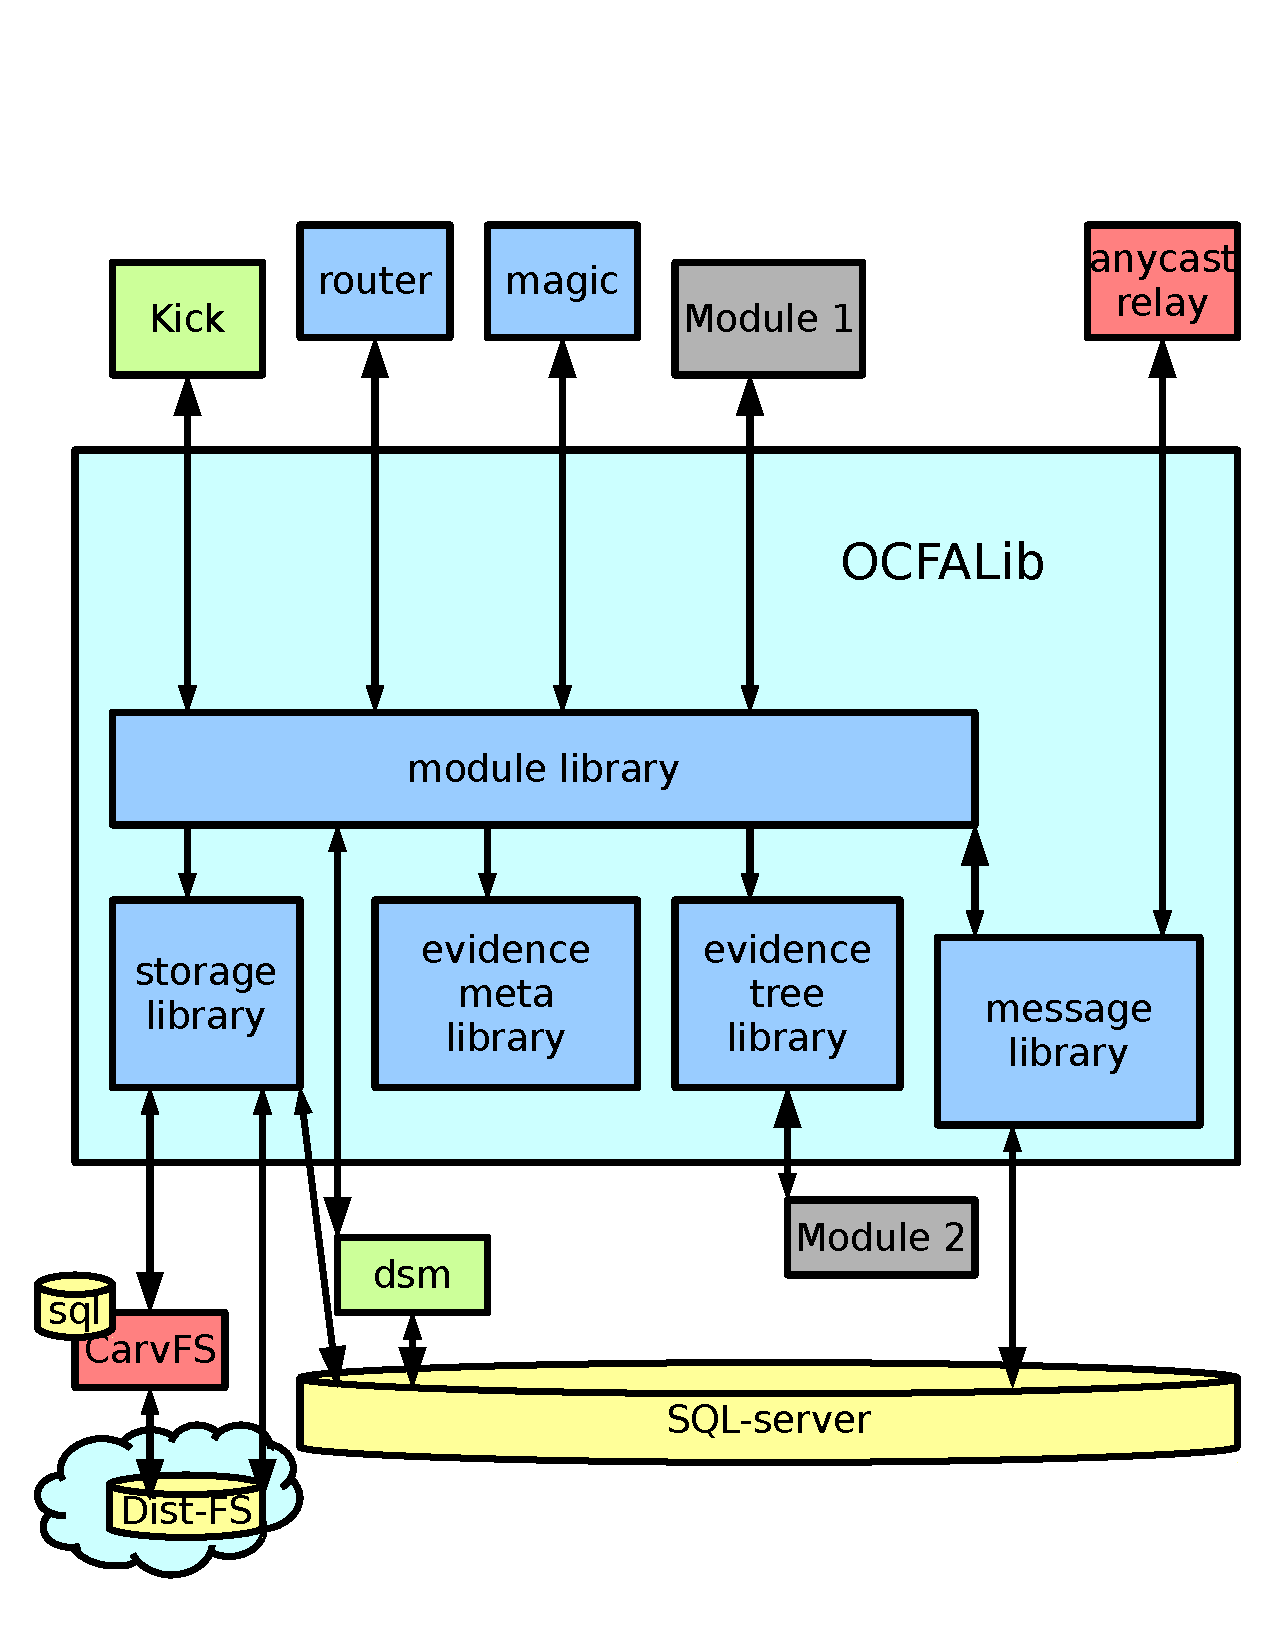
\includegraphics[width=100mm]{mattock/libraryview.pdf}
\caption{The base OCFA architecture}
\label{fig:FlowInOut}
\end{figure}
\subsection{The AnyCast Relay and Persistent Priority Queue}
\subsection{OcfaLib, a domain specific asynchonous framework}
\subsection{The lagacy Module API}
\subsection{The Treegraph API}
\subsection{The legacy CAS storage}
\subsection{CarvFS}
\subsection{The meta-data based message router}
\subsection{The use of an SQL server}
\section{New insights}
\section{A modernized architecture}
\begin{figure}
\centering
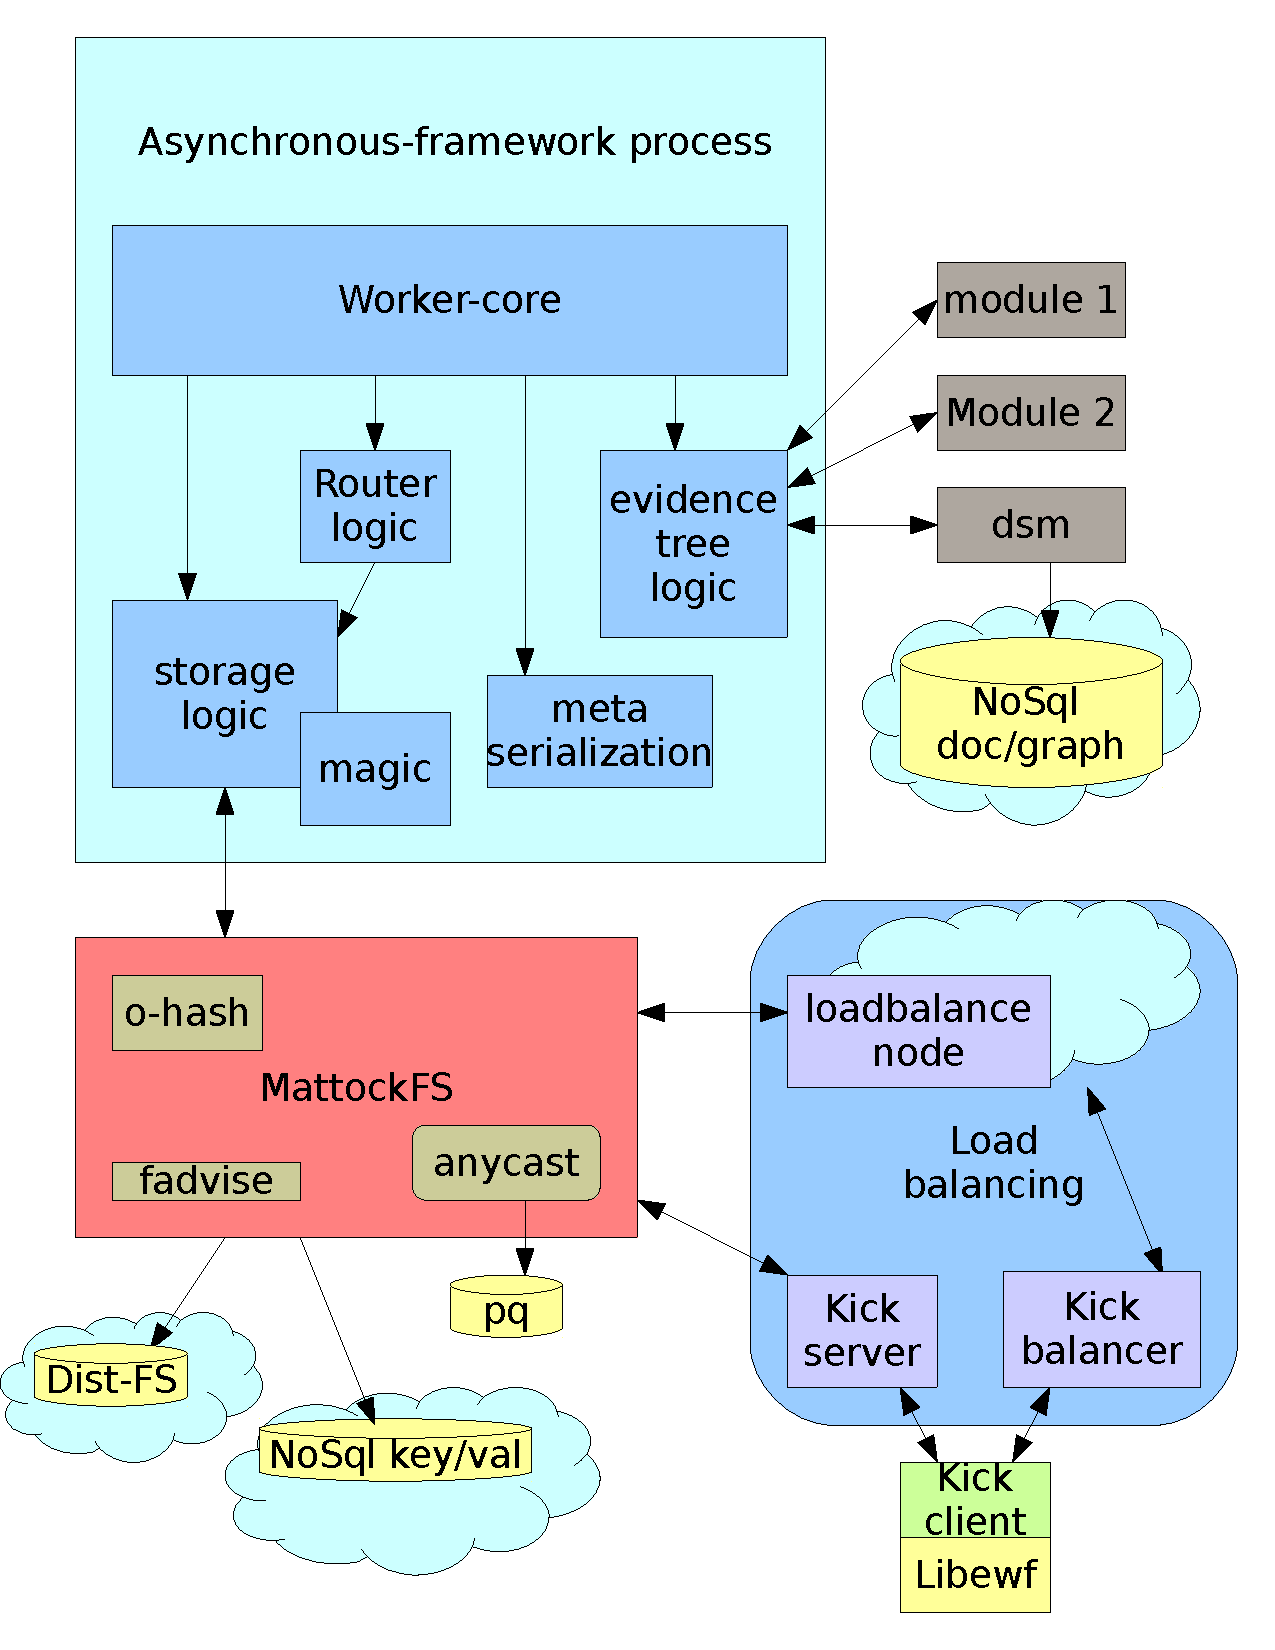
\includegraphics[width=100mm]{mattock/libraryviewmattock.pdf}
\caption{The base Mattock architecture}
\label{fig:FlowInOut}
\end{figure}
\subsection{MattockFS \& the distributed longpath store}
\subsection{The AnyCast meshup}
\subsection{Client/Server kickstarting}
\subsection{Effective distributed system usage}
\subsection{Store-system embedded libmagic functionality}
\subsection{Distributed routing logic}
\subsection{From SQL to Document/Graph based NoSQL}
\subsection{Using language-native asynchonous frameworks}
\subsection{A single tree-graph, lambda and asynchonous operation oriented API}
\subsection{Conclusion}
